%%%%%%%%%%%%%%%%%%%%%%%%%%%%%%%%%%%%%%%%%%%%%%%%%%%%%%%%%%%%%%%%%%%%
% This is a thesis template for Gebze Technical University.
%
% Please only edit the areas proceeded by a comment starting with %%
% otherwise the template may be broken.
%
% This file is only to be used for editing the general fields
% and inputting the body of the thesis in the designated areas.
% Please write the body of the thesis in separate files, and input
% them as shown in the comment preceding the area.
%
% Created in Aug 2021 by Usama Derbashi.
%%%%%%%%%%%%%%%%%%%%%%%%%%%%%%%%%%%%%%%%%%%%%%%%%%%%%%%%%%%%%%%%%%%%
\documentclass[12pt]{report}


% Language and typeset setting
\usepackage[english]{babel}
\usepackage[a4paper,top=25mm,bottom=25mm,left=40mm,right=25mm]{geometry}
\usepackage[onehalfspacing]{setspace}
\usepackage{algorithm, algpseudocode}
\usepackage{indentfirst}
\setlength{\parindent}{1cm}
\setlength{\abovecaptionskip}{12pt plus 0pt minus 0pt}
\setlength{\belowcaptionskip}{12pt plus 0pt minus 0pt}
\setlength{\textfloatsep}{18.0pt plus 0.0pt minus 0.0pt}
\setlength{\floatsep}{18.0pt plus 0.0pt minus 0.0pt}
\setlength{\intextsep}{18.0pt plus 0.0pt minus 0.0pt}
\setlength{\skip\footins}{18.0pt plus 0.0pt minus 0.0pt}

% Core packages and settings
\usepackage[colorlinks=false]{hyperref}
\usepackage{amsmath}

\usepackage{titlesec} %setting the titles of chapters and sections
\setcounter{secnumdepth}{4}
\setcounter{tocdepth}{4}
\titleformat{\chapter}[hang]{\normalfont\bfseries\MakeUppercase}{}{0pt}{\LARGE\thechapter. }
\titleformat{\section}[hang]{\normalfont\bfseries}{}{0pt}{\Large\thesection. }
\titleformat{\subsection}[hang]{\normalfont\bfseries}{}{0pt}{\large\thesubsection. }
\titleformat{\subsubsection}[hang]{\normalfont\bfseries}{}{0pt}{\large\thesubsubsection. }
\titlespacing*{\chapter}{0pt}{0pt}{18pt}
\titlespacing*{\section}{0pt}{18pt}{18pt}
\titlespacing*{\subsection}{0pt}{18pt}{18pt}
\titlespacing*{\subsubsection}{0pt}{18pt}{18pt}

\usepackage{graphicx}
\graphicspath{{./Imgs/}} %pointing the directory of images

\usepackage{fancyhdr} % setting footers
\usepackage{etoolbox} 
\renewcommand{\headrulewidth}{0pt}
\patchcmd{\chapter}{\thispagestyle{plain}}{\thispagestyle{fancy}}{}{}
\pagestyle{fancy}
\fancyhf{}
\fancyfoot[C]{\fontsize{11pt}{11pt}\thepage}

\usepackage[style=ieee]{biblatex}
\addbibresource{refs.bib}
\usepackage{csquotes}% Needed for babel(in biblatex)

\usepackage[bottom, perpage]{footmisc}%% amkes footnotes at the bottom

\usepackage{GTUThesis}


% Additional packages if needed
%% For the sake of not messing the template add them here
\usepackage{lipsum}

\usepackage{tikz}
\usetikzlibrary{shapes.geometric, arrows}

\tikzstyle{actor} = [draw, ellipse, minimum width=3cm, minimum height=1cm, text centered, draw=black, fill=red!30]
\tikzstyle{usecase} = [ellipse, draw=blue, fill=blue!20, text centered, minimum width=3cm, minimum height=1cm, text width=2cm]


% Important information
%% Make sure to enter all the info below
\title{AR Based Quality Control System On VisionPro}
\author{
    BİLAL GÖKÇE 
	\linebreak
    MELİKE SEYİTOĞLU
}
\faculty{Faculty of Engineering}
\department{Computer Engineering Department}
\supervisor{Dr. Yakup GENÇ}
\theyear{2025}


\begin{document}

%Front Matter
\pagenumbering{roman} %start with roman numbering 
\projecttitlepageenglish
\maketitle
\setcounter{page}{3} %the first two title pages are not counted so this is a buffer
\begin{outertitles} % makes titles centred

%% below enter as follows 
%% {DATE_OF_DEMO}{JURY}
%% Note that JURY should be comma separated
\makejury{../../2025}{Prof. Dr. Yusuf Sinan AKGÜL}

\chapter*{Abstract}
\addcontentsline{toc}{chapter}{Abstract}

%% Edit below this line
In this project, we adapted an existing quality control system for the iPad to the Apple Vision Pro (AVP) The application features several core functionalities, including UI/UX design, ground detection, AR object placement and replacement, inspection of designated points, and the ability to generate reports.

We evaluated the success of our system by investigating and analyzing its performance based on speed and efficiency.
%% Until here
\vfill
%% Edit after {Keywords:}
\textbf{Keywords:} AVP, UI/UX, AR.
\clearpage
\chapter*{Acknowledgement}
\addcontentsline{toc}{chapter}{Acknowledgement}

We would like to express our deepest gratitude to our advisor, Dr. Yakup GENÇ, for his support in providing us access to the Apple Vision Pro and related devices, as well as the invaluable opportunities that have greatly contributed to the success of this project.

\vspace{1cm}
\begin{flushright}
    BİLAL GÖKÇE \\
    MELİKE SEYİTOĞLU \\
\end{flushright}
\begin{flushleft}
    January, 2025
\end{flushleft}
\clearpage
\chapter*{List of Symbols and Abbreviations}
\addcontentsline{toc}{chapter}{List of Symbols and Abbreviations}

\begin{tabular}{lcl}
    \textbf{Symbol or}&&\\
    \textbf{Abbreviation} &:& \textbf{Explanation}\\
    
    AR &:& Augmented Reality\\
    AVP &:& Apple Vision Pro\\
    ARKit &:& Apple's Augmented Reality Framework\\
    UI &:& User Interface\\
    UX &:& User Experience\\
    USDZ &:& Universal Scene Description (3D File Format)\\
    libxlsxwriter &:& A C library for creating Excel files\\
    FPS &:& Frames Per Second\\
    ms &:& Milliseconds\\
    $t_{avg}$ &:& Average Latency\\
    ML &:& Machine Learning\\
    CAD &:& Computer-Aided Design\\
    SceneKit &:& Apple’s 3D Graphics Framework\\
    GPU &:& Graphics Processing Unit\\
    
\end{tabular}

\clearpage


\tableofcontents
\addcontentsline{toc}{chapter}{Contents}
\clearpage

\listoffigures
\addcontentsline{toc}{chapter}{List of Figures}
\clearpage

\listoftables
\addcontentsline{toc}{chapter}{List of Tables}
\clearpage



\end{outertitles}
\fancyhf{}%reset footer
\fancyfoot[R]{\fontsize{11pt}{11pt}\thepage}%page numbers in the corner
\addtocontents{toc}{\protect\vspace{18pt}}
\pagenumbering{arabic}%turn to arabic numbers

% Mainmatter

%% Only input files, don't write here
%% \input{./Body/Mainmatter/FILE}
\chapter{Introduction}

Augmented reality (AR) technologies have revolutionized various industries, offering innovative solutions to complex problems. Quality control systems are one such area where AR can provide immense value. While similar applications exist on platforms like the iPad, their limitations in spatial capabilities and less intuitive interaction methods make them less suitable for high-precision tasks. In this project, we have developed a quality control system tailored for the Apple Vision Pro (AVP), leveraging its advanced spatial capabilities, immersive experience, and intuitive gesture-based controls.

Our solution addresses the limitations of traditional systems by integrating advanced features such as 3D CAD model alignment, real-time object tracking, and automated reporting. These enhancements make the AVP-based quality control system ideal for industries demanding high precision and efficiency.

\section{Project Definition}

The aim of this project is to develop a quality control system specifically designed for the Apple Vision Pro (AVP). Unlike iPads, which have limited spatial features, the AVP offers advanced spatial capabilities and immersive interaction methods that make it ideal for high-precision tasks. This system leverages the AVP’s strengths to improve accuracy and efficiency in quality control processes.

The key functionalities include aligning 3D CAD models with real-world objects, enabling interactive inspections at predefined points, and generating detailed quality analysis reports. By addressing the limitations of tablet-based systems, this project aims to provide an innovative solution for industries requiring precise quality control.


% This project focuses on designing and implementing a quality control system for the Apple Vision Pro (AVP). The system utilizes the AVP's cutting-edge spatial and interaction capabilities to enhance accuracy and user experience. The core functionality revolves around:
% \begin{itemize}
%     \item Aligning 3D CAD models with real-world objects to identify differences.
%     \item Providing users with tools for interactive and natural inspection using gesture-based controls.
%     \item Generating quality analysis reports in Excel format for documentation and review.
%     \item Allowing users to inspect predefined points on models for detailed quality control.
% \end{itemize}

% During the inspection process, users can select specific inspection points on the model to perform quality checks. These inspections can include:
% \begin{itemize}
%     \item Yes/No Verification: Confirming whether a feature meets the required specifications.
%     \item Description-based Analysis: Providing detailed notes about the inspected feature.
%     \item Count-based Evaluation: Counting the number of specific elements.
% \end{itemize}

% The application is designed to support industries where precise quality control is critical, such as manufacturing, automotive, and aerospace.

\section{Project Aims}

The primary aims of this project are as follows:
\begin{enumerate}
    \item \textbf{Enhanced User Experience:} Develop an intuitive UI/UX interface with gesture-based controls, including eye-tracking and finger interactions.
    \item \textbf{Precise Model Alignment:} Implement a robust algorithm for aligning 3D CAD models with real-world objects, ensuring high accuracy.
    \item \textbf{Inspection Points:} Enable users to select and inspect specific points on models, offering flexible options like yes/no, descriptions, and counts for quality control.
    \item \textbf{Automated Reporting:} Create a reporting feature that allows users to extract detailed quality analysis in Excel format.
    \item \textbf{Performance Optimization:} Ensure the system operates efficiently, achieving high frame rates, low latency, and inspection speeds comparable to or better than tablet-based solutions.
\end{enumerate}

These aims are designed to address the current limitations of traditional quality control systems and utilize the advanced capabilities of the Apple Vision Pro to deliver an innovative and efficient solution.

\chapter{Project Details}

This chapter provides an in-depth explanation of the project's components and tools used. The system was developed using Swift, Xcode, and RealityComposer Pro to leverage the capabilities of Apple Vision Pro.

% \section{UI/UX Design}
\section{UI/UX Design}

The application has a streamlined user interface with a single window navigating between different views to ensure an intuitive and user-friendly experience. Below is the flow of UI/UX interactions:

\subsection{Initial Session Start}
The application starts with a view prompting the user to begin an ARKit session. This session initializes plane detection and world tracking. The interface provides visual indicators to guide the user during this setup phase. (Figure \ref{fig:ui_session_start} shows the UI at this stage.)
\begin{figure}[h!]
    \centering
    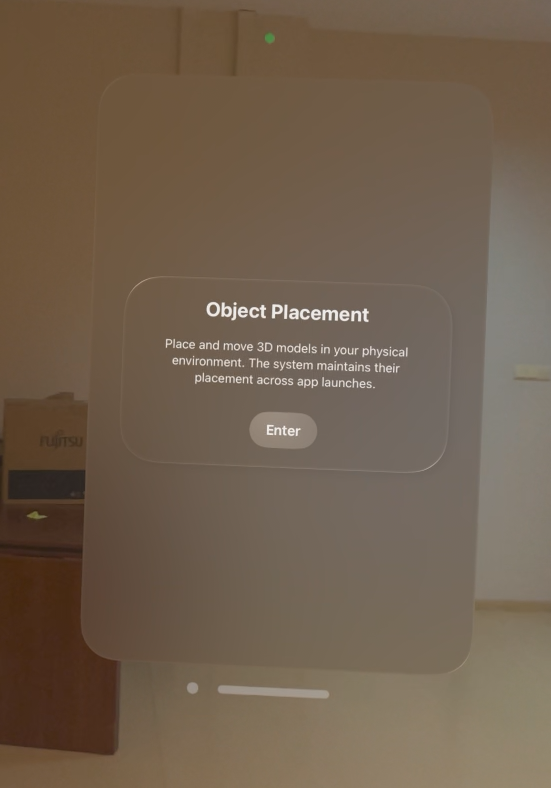
\includegraphics[width=0.4\textwidth]{session_start_ui.png} % Replace with your image file name
    \caption{UI for starting the ARKit session.}
    \label{fig:ui_session_start}
\end{figure}
\subsection{Object Selection Menu}
After initializing the session, the user is directed to an object selection menu. In this view:
\begin{itemize}
    \item The user selects an object from the available options.
    \item When an object is clicked, the \texttt{selectedObject} state is updated.
    \item The selected object is prepared for placement. (Figure \ref{fig:ui_object_selection} shows the object selection menu.)
\end{itemize}
\begin{figure}[h!]
    \centering
    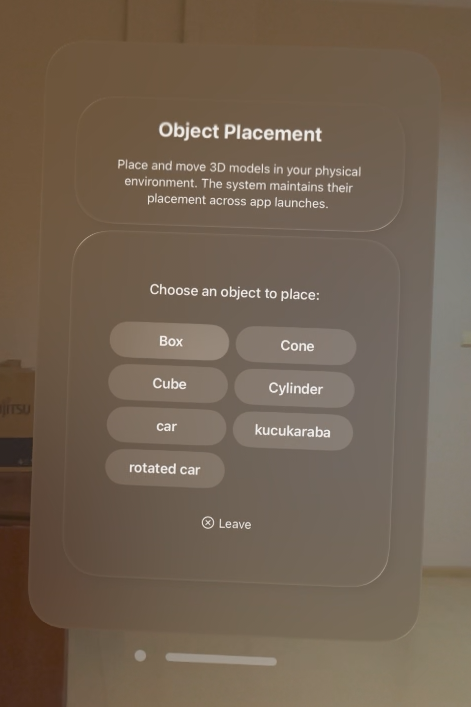
\includegraphics[width=0.4\textwidth]{object_selection_ui.png} % Replace with your image file
    \caption{Object selection menu UI.}
    \label{fig:ui_object_selection}
\end{figure}

\subsection{Initial Object Placement}
During the initial placement of the selected object:
\begin{itemize}
    \item Placement tooltips are displayed to guide the user on positioning the object accurately.
    \item Visual aids ensure the user understands how to interact with the AR environment. (Figure \ref{fig:ui_initial_placement} shows the placement tooltip.)
\end{itemize}
\begin{figure}[h!]
    \centering
    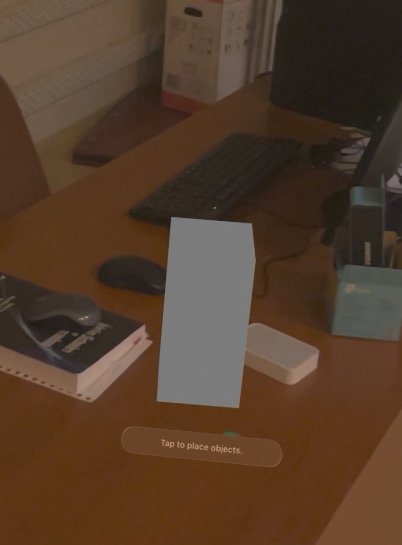
\includegraphics[width=0.4\textwidth]{object_placement_tooltips.png} % Replace with your image file
    \caption{Placement tooltips during initial object placement.}
    \label{fig:ui_initial_placement}
\end{figure}


\subsection{Object Interaction View}
If there is already a placed object, the application navigates directly to the object interaction view. In this view:
\begin{itemize}
    \item The user can perform repositioning, inspection, or removal of the placed object. The interface displays three buttons for these actions, as shown in Figure \ref{fig:ui_three_buttons}.
    \begin{figure}[h!]
        \centering
        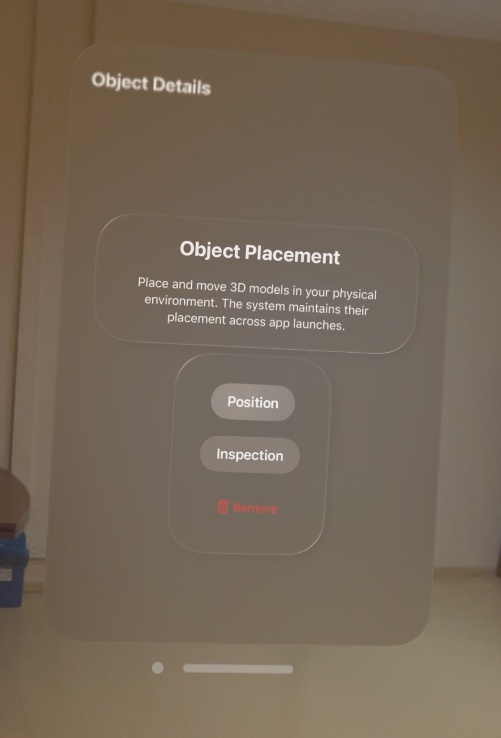
\includegraphics[width=0.39\textwidth]{three_buttons_ui.png} % Replace with the actual file name
        \caption{UI showing the three buttons for repositioning, inspection, and removal.}
        \label{fig:ui_three_buttons}
    \end{figure}
    \clearpage
    \item Three buttons allow the user to activate these actions:
    \begin{itemize}
        \item \textbf{Repositioning:} Includes rotation, left/right movement, and forward/backward movement. The user can use pinch and drag gestures (thumb and index finger) to perform the action. Only one action can be performed at a time. (Figure \ref{fig:ui_repositioning} shows the repositioning process.)
        \begin{figure}[h!]
            \centering
            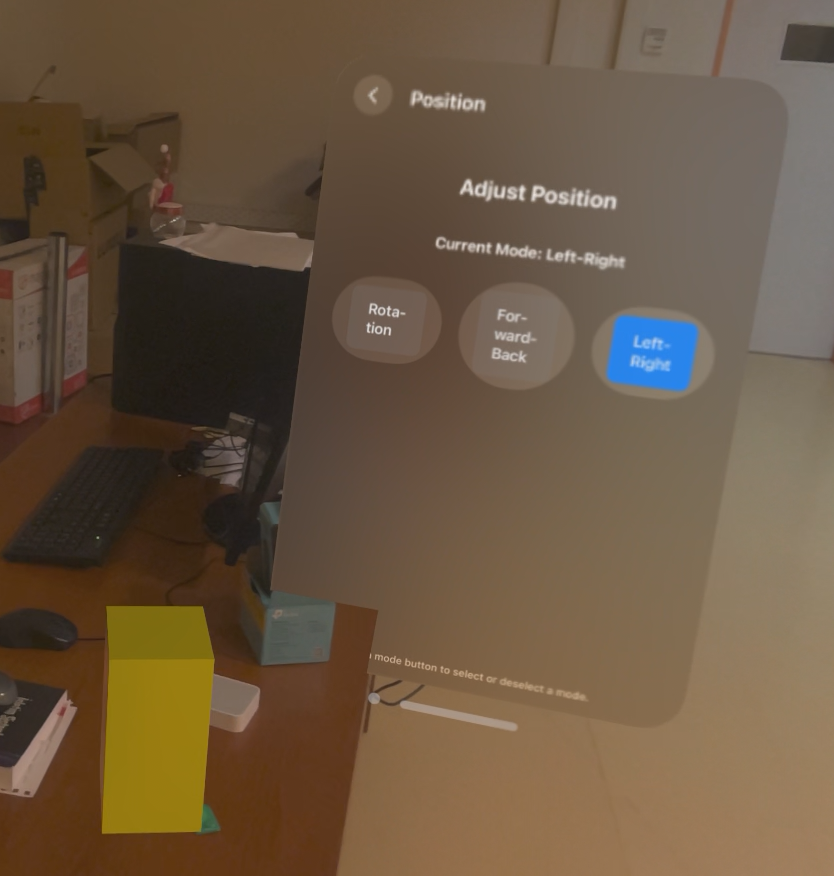
\includegraphics[width=0.6\textwidth]{repositioning_ui.png} % Replace with the actual file name
            \caption{Repositioning the object using pinch and drag gestures.}
            \label{fig:ui_repositioning}
        \end{figure}
        \item \textbf{Inspection:} Inspection points are UI buttons attached to the placed object. These points activate only in the inspection view. In addition, the inspection view includes a \textbf{Generate Report} button, allowing the user to extract detailed quality analysis reports based on the performed inspections. (Figure \ref{fig:ui_inspection_view} shows the inspection view.)
        \clearpage
        \begin{figure}[h!]
            \centering
            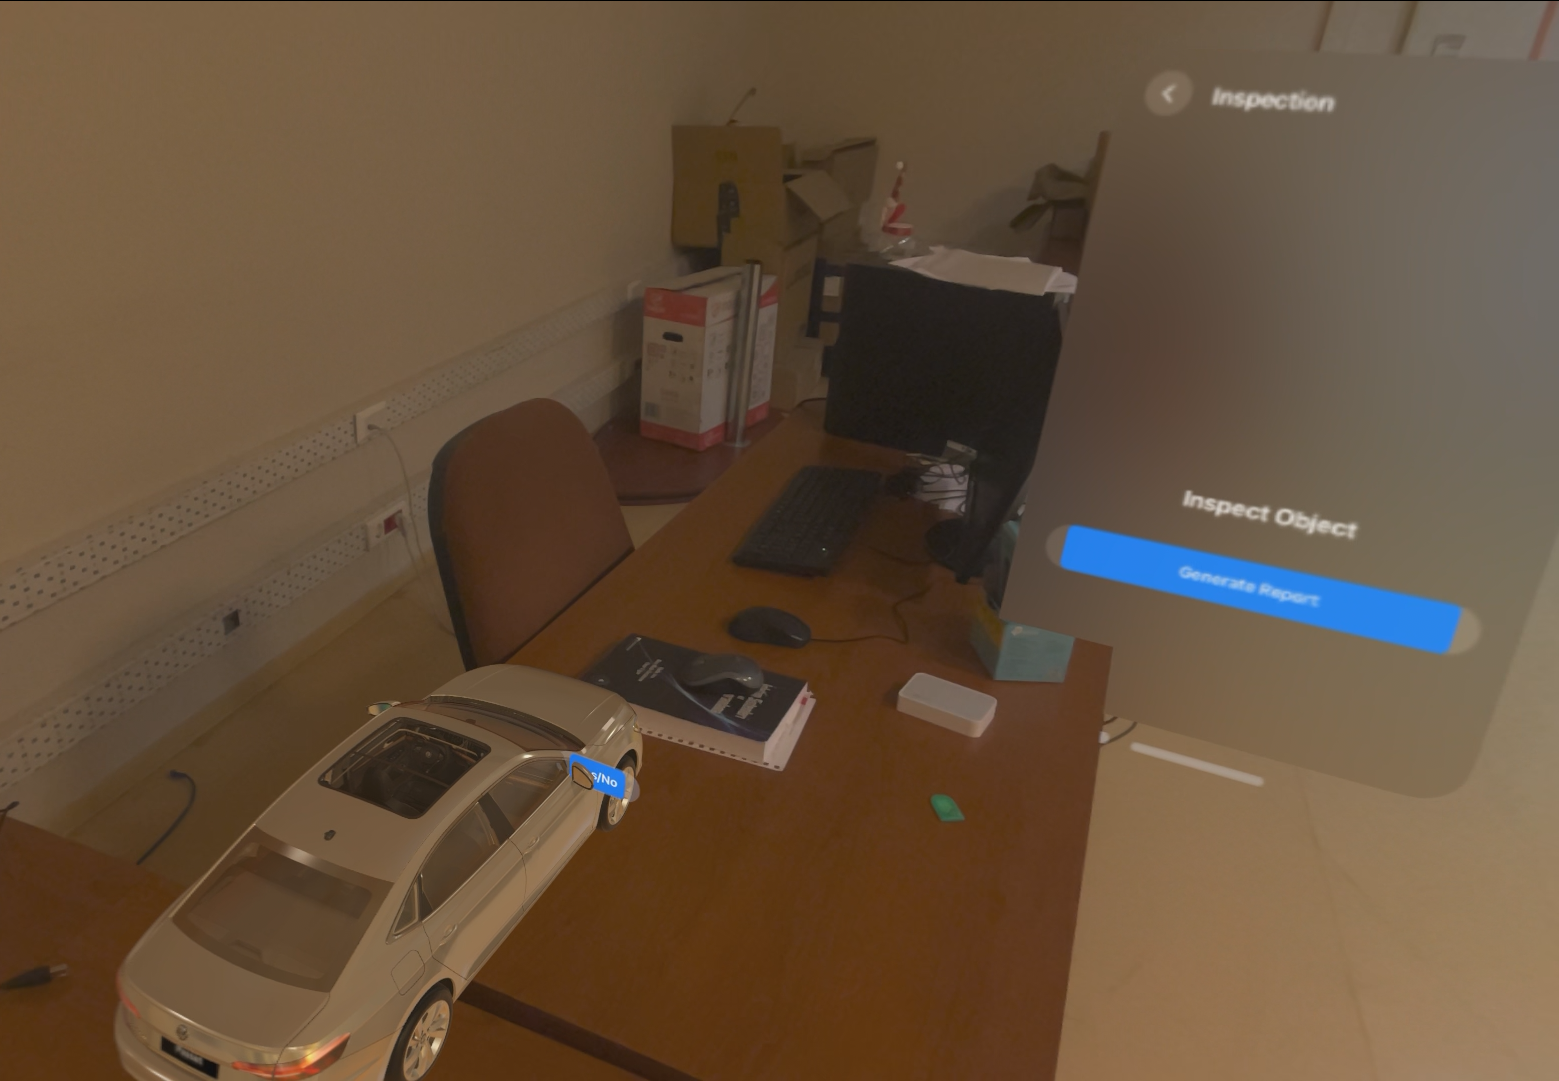
\includegraphics[width=0.8\textwidth]{inspection_view_ui.png} % Replace with the actual file name
            \caption{Inspection view showing active inspection points.}
            \label{fig:ui_inspection_view}
        \end{figure}
        \item \textbf{Removal:} To remove the placed object, the user presses the remove button. A confirmation popup appears to ensure the action is intentional. (Figure \ref{fig:ui_remove_popup} shows the removal confirmation popup.)
        \begin{figure}[h!]
            \centering
            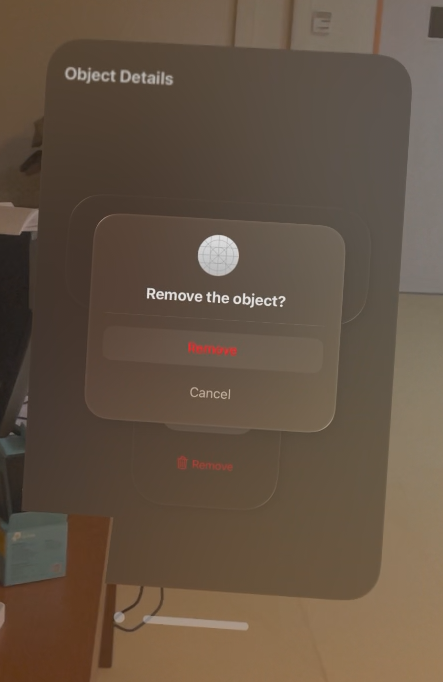
\includegraphics[width=0.4\textwidth]{remove_popup_ui.png} % Replace with the actual file name
            \caption{Confirmation popup for removing the placed object.}
            \label{fig:ui_remove_popup}
        \end{figure}
    \end{itemize}
\end{itemize}

\subsection{Inspection Detail View}
When an inspection point is clicked, the application navigates to the inspection detail view:
\begin{itemize}
    \item A question specific to the inspection point is displayed, which can be one of the following:
    \begin{itemize}
        \item Yes/No question.
        \item Count input.
        \item Description input.
    \end{itemize}
    \item The user provides the required input or feedback. (Figure \ref{fig:ui_inspection_detail} shows the inspection detail view.)
\end{itemize}

\begin{figure}[h!]
    \centering
    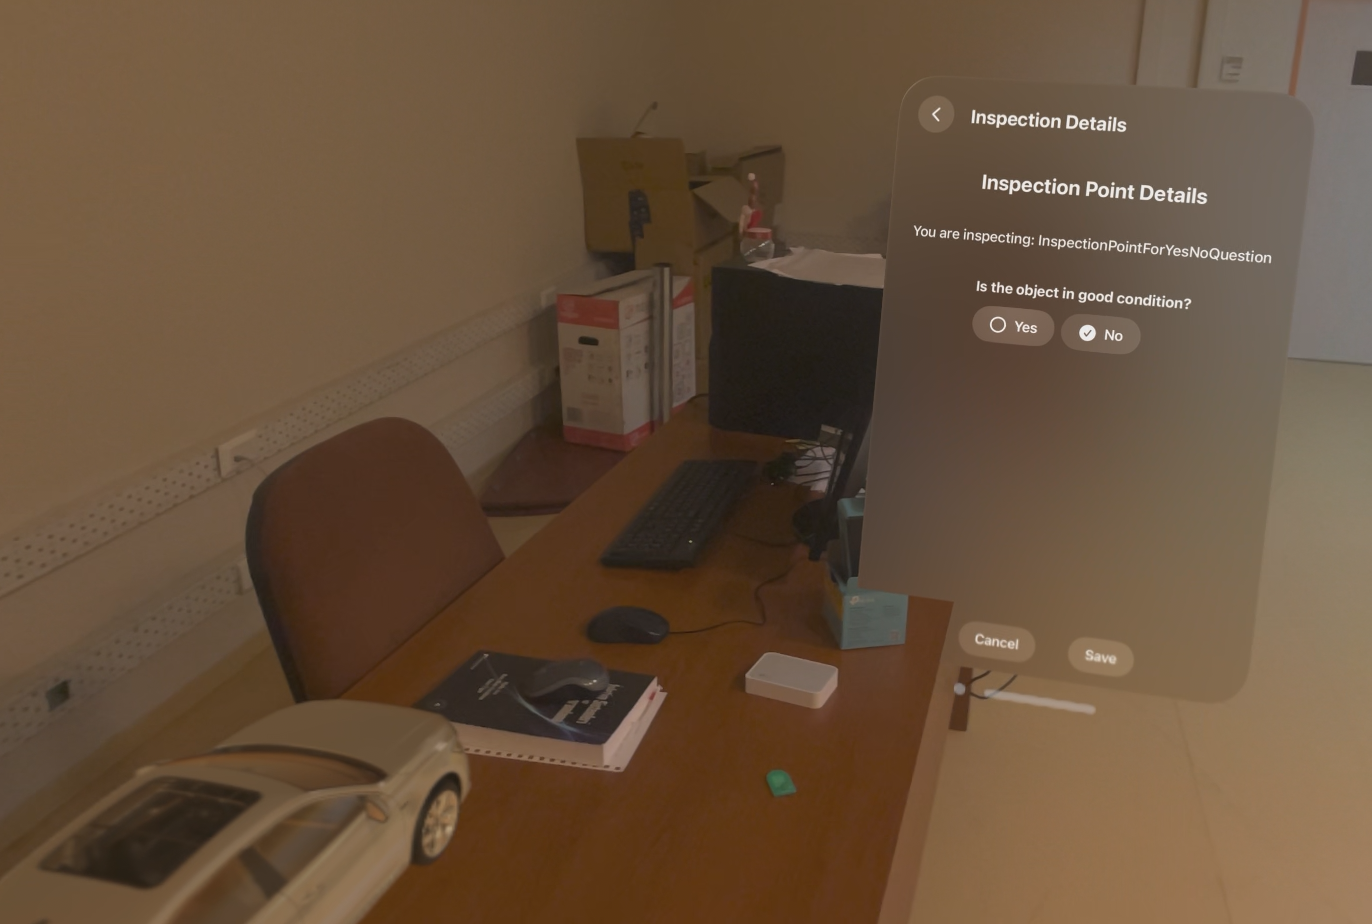
\includegraphics[width=0.8\textwidth]{inspection_detail_ui.png} % Replace with your actual file name
    \caption{Inspection detail view showing specific question types and input fields.}
    \label{fig:ui_inspection_detail}
\end{figure}


\section{Model Alignment and Placement}

The system leverages ARKit’s capabilities for world tracking and plane detection to enable accurate model alignment and placement. Horizontal planes are specifically chosen to detect ground planes, ensuring precise object placement in the AR environment.

The 3D models used in the application are in the USDZ format, which is optimized for AR experiences on Apple devices.
\subsection{Initial Placement}
During initial placement, the user is provided with a preview of the selected object. The preview is displayed as a greyed-out version of the object accompanied by a placement tooltip to guide the user in positioning it accurately. This feature allows the user to visually align the object with the detected ground plane before finalizing its placement, as shown in Figure \ref{fig:ui_initial_placement}.

To ensure that objects fit appropriately within the environment, size adjustments are made to the USDZ 3D models using SceneKit. 
\subsection{Replacement}
If the user needs to reposition an already placed object, they can do so in the position mode of the application. In this mode:
\begin{itemize}
    \item The user can perform object rotation, as well as left/right and forward/backward movements.
    \item These adjustments are enabled only when the position mode is activated in the position view.
    \item Pinch and drag gestures (thumb and index finger) are used to perform these actions, as shown in \ref{fig:ui_repositioning}.
\end{itemize}

By combining ARKit’s robust plane detection with intuitive interaction methods, the system ensures precise and user-friendly model alignment and placement.


% Explanation about inspection will go here.
\section{Inspection}

All inspection operations, including exporting reports, providing input to inspection points, or viewing inspection points, occur exclusively within the \textbf{Inspection View}. If the application is not in the \textbf{Inspection View}, all inspection points are removed from the interface. When the user navigates back to the \textbf{Inspection View}, the inspection points are dynamically regenerated. (as shown in Figure \ref{fig:ui_inspection_view})

To prevent user confusion or potential issues (e.g., uncertainty about whether data is saved), all inspection points are also removed when the application navigates to the \textbf{Inspection Detail View}. This design decision ensures reliability and eliminates bugs arising from unclear save states or interactions. (as Shown in Figure \ref{fig:ui_inspection_detail})

\subsection{Inspection Points}
For each inspection point on the placed model, a UI button is displayed (as shown in Figure \ref{fig:ui_inspection_view}). These buttons are dynamically positioned based on the specific locations of the inspection points on the model. When the user clicks an inspection point button, the application navigates to the \textbf{Inspection Detail View}, where the selected inspection point can be reviewed and updated.

\subsection{Inspection Detail View}
In the \textbf{Inspection Detail View}, users can perform inspections on the selected point. The system supports three types of inspections:
\begin{itemize}
    \item \textbf{Yes/No:} A binary choice indicating whether the inspection criteria have been met, as Shown in Figure \ref{fig:ui_inspection_detail}.
    \item \textbf{Count:} Allows the user to input the quantity of specific elements related to the inspection point.
    \item \textbf{Description:} Provides a text field for the user to enter detailed notes or comments about the inspection point.
\end{itemize}

\subsection{Exporting Reports}
The \textbf{Inspection View} includes a \textbf{Generate Report} button, enabling users to export a report of all completed inspections.

By limiting inspection operations to the \textbf{Inspection View} and \textbf{Inspection Detail View}, the system ensures a consistent and reliable user experience while minimizing potential errors or confusion.


% Explanation about generating reports will go here.
\section{Report Generation}

The report generation functionality in this system is powered by the third-party C library \textbf{libxlsxwriter}, which facilitates the creation of Excel files. This feature enables users to export inspection reports, which are saved directly to the Apple Vision Pro's local directory for easy access.

\subsection{Implementation Overview}
Each report file is named dynamically based on the object being inspected and a unique identifier to avoid conflicts.

\subsection{Report Content}
The generated report contains the following key information:
\begin{itemize}
    \item \textbf{Object Details:} The name, width, height, and depth of the inspected object are recorded in the report.
    \item \textbf{Inspection Points:} Each inspection point associated with the object is detailed in the report. For every inspection point, the following attributes are included:
    \begin{itemize}
        \item \textbf{Name:} The identifier of the inspection point.
        \item \textbf{Depending on The Type of Inspection:}
        \begin{itemize}
            \item \textbf{Count:} The quantity associated with the inspection point, if applicable.
            \item \textbf{Description:} Detailed notes or observations provided by the user.
            \item \textbf{Is Correct:} A binary value (Yes/No) indicating whether the inspection point meets the desired criteria.
        \end{itemize}
    \end{itemize}
\end{itemize}

An example of the generated Excel report is shown in Figure \ref{fig:example_excel}.
\begin{figure}[h!]
    \centering
    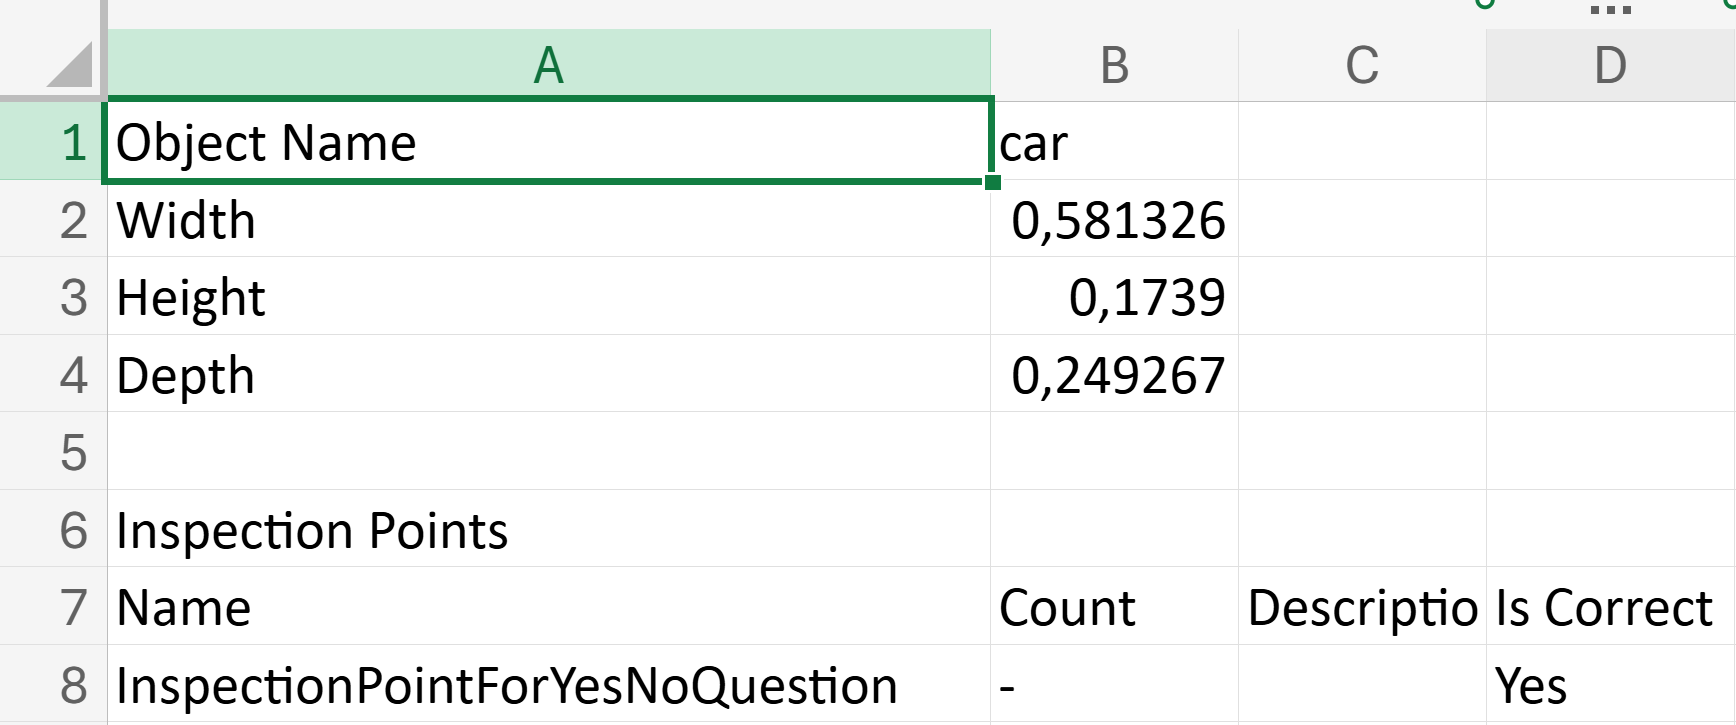
\includegraphics[width=0.8\textwidth]{example_excel.png} % Replace with your actual file name
    \caption{Example Excel report generated by the application.}
    \label{fig:example_excel}
\end{figure}

\subsection{Integration with Apple Vision Pro}
The reports are stored locally on the Apple Vision Pro device, allowing users to access them conveniently through the file system. This integration ensures compatibility with the Vision Pro environment and leverages the device's capabilities for efficient data handling.

By using \textbf{libxlsxwriter}, the system provides a robust and efficient way to generate and manage detailed Excel reports, enhancing the overall functionality and usability of the quality control application.



\section{Use Case Diagram}
The use case diagram below illustrates the interaction between the user and the primary functionalities of the system.

\begin{center}
    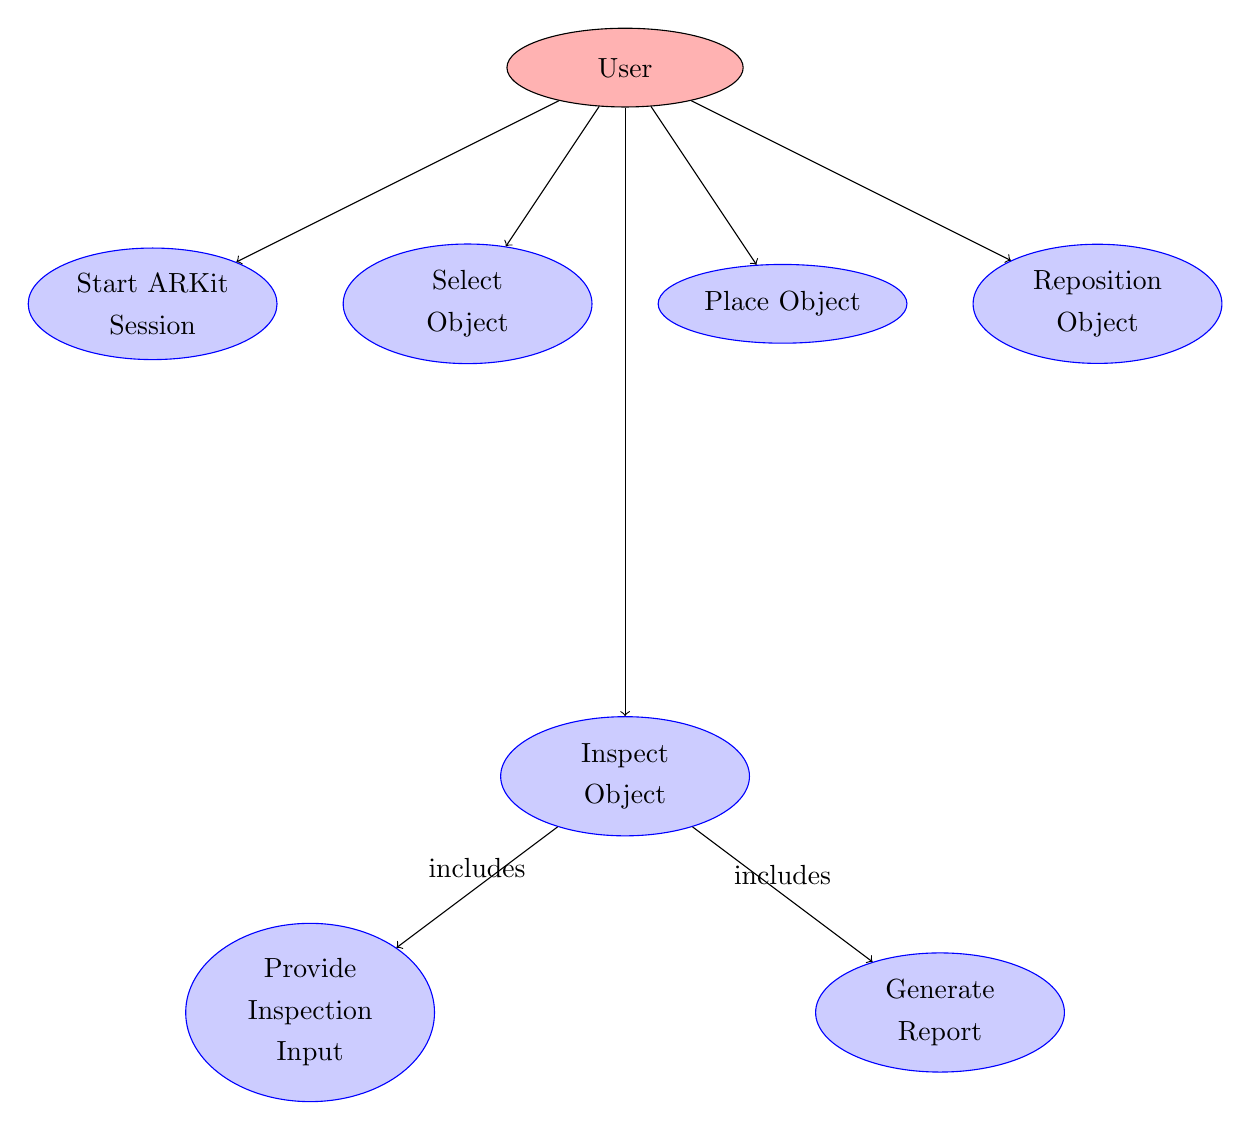
\begin{tikzpicture}[node distance=3cm]

        % Actor
        \node (user) [actor] {User};

        % Use cases
        \node (start) [usecase, below of=user, xshift=-6cm] {Start ARKit Session};
        \node (select) [usecase, below of=user, xshift=-2cm] {Select Object};
        \node (place) [usecase, below of=user, xshift=2cm] {Place Object};
        \node (reposition) [usecase, below of=user, xshift=6cm] {Reposition Object};
        \node (inspect) [usecase, below of=user, yshift=-6cm] {Inspect Object};
        \node (provide) [usecase, below of=inspect, xshift=-4cm] {Provide Inspection Input};
        \node (report) [usecase, below of=inspect, xshift=4cm] {Generate Report};

        % Connections between actor and use cases
        \draw [->] (user) -- (start);
        \draw [->] (user) -- (select);
        \draw [->] (user) -- (place);
        \draw [->] (user) -- (reposition);
        \draw [->] (user) -- (inspect);

        % Relationships between use cases
        \draw [->] (inspect) -- node[midway, above] {includes} (provide);
        \draw [->] (inspect) -- node[midway, above] {includes} (report);

    \end{tikzpicture}
\end{center}


\chapter{Conclusion and Results}

This chapter presents the evaluation of the quality control system based on the predefined success criteria: \textbf{inspection efficiency} and \textbf{low latency}. The results demonstrate the performance of the system and its ability to meet the intended objectives.

\section{Inspection Efficiency}

The inspection efficiency of the system was evaluated by comparing the time required to perform specific tasks on a traditional tablet versus the Apple Vision Pro (AVP). The results are summarized in Table \ref{tab:inspection_efficiency}.

\begin{table}[h!]
    \centering
    \caption{Inspection Efficiency Comparison}
    \label{tab:inspection_efficiency}
    \begin{tabular}{|l|c|c|c|}
        \hline
        \textbf{Task} & \textbf{Tablet Time (s)} & \textbf{AVP Time (s)} & \textbf{Efficiency (\%)} \\
        \hline
        1 Description Inspection & 30 & 36 & 83.3 \\
        1 Description + 2 Yes/No Inspections & 37 & 45 & 82.2 \\
        \hline
    \end{tabular}
\end{table}

\subsection{Analysis of Results}
The efficiency percentage was calculated using the following formula:
\[
\text{Efficiency (\%)} = \frac{\text{Tablet Time}}{\text{AVP Time}} \times 100
\]

From the table, we can observe:
\begin{itemize}
    \item For \textbf{Alignment + 1 Description Inspection}, the system achieved an efficiency of \textbf{83.3\%}.
    \item For \textbf{Alignment + 1 Description + 2 Yes/No Inspections}, the system achieved an efficiency of \textbf{82.2\%}.
\end{itemize}

\subsection{Conclusion on Inspection Efficiency}
While the system did not meet the target of achieving at least 95\% of the inspection speed compared to a tablet, the results indicate that the AVP-based system maintains a reasonable level of performance. Using the AVP for this application, particularly the chosen UI design, is slowing down the process. However, the system's efficiency is still acceptable for practical use.

\section{Latency Results}

The latency of various operations was measured to evaluate the system's performance. The results are presented below, categorized by operation type.

\subsection{Latency in Update Placement}
The latency values for updating placements are summarized in Table \ref{tab:update_placement_latency}. The average latency was calculated as the mean of all recorded values.

\begin{table}[h!]
    \centering
    \caption{Latency Results for Update Placement}
    \label{tab:update_placement_latency}
    \begin{tabular}{|c|c|}
        \hline
        \textbf{Test Number} & \textbf{Latency (seconds)} \\
        \hline
        1 & 0.0001039505 \\
        2 & 0.0001161098 \\
        3 & 0.0001189709 \\
        4 & 0.0001029968 \\
        5 & 0.0001029968 \\
        6 & 0.0001230240 \\
        7 & 0.0000960827 \\
        8 & 0.0000970364 \\
        9 & 0.0000998974 \\
        10 & 0.0001351833 \\
        11 & 0.0001239777 \\
        12 & 0.0001008511 \\
        13 & 0.0001068115 \\
        14 & 0.0001409054 \\
        15 & 0.0001020432 \\
        16 & 0.0001068115 \\
        17 & 0.0001428127 \\
        18 & 0.0002100468 \\
        19 & 0.0004167557 \\
        20 & 0.0001139641 \\
        \hline
        \multicolumn{1}{|r|}{\textbf{Average Latency:}} & \textbf{0.0001325284} \\
        \hline
    \end{tabular}
\end{table}

\subsection{Latency in Object Selection}
The latency values for object selection are presented in Table \ref{tab:object_selection_latency}.

\begin{table}[h!]
    \centering
    \caption{Latency Results for Object Selection}
    \label{tab:object_selection_latency}
    \begin{tabular}{|c|c|}
        \hline
        \textbf{Test Number} & \textbf{Latency (seconds)} \\
        \hline
        1 & 0.0004739761 \\
        2 & 0.0004129410 \\
        3 & 0.0006000996 \\
        4 & 0.0004827976 \\
        5 & 0.0120141506 \\
        6 & 0.0209228992 \\
        7 & 0.0204608440 \\
        8 & 0.0109148026 \\
        9 & 0.0004229546 \\
        10 & 0.0017952919 \\
        \hline
        \multicolumn{1}{|r|}{\textbf{Average Latency:}} & \textbf{0.0064594758} \\
        \hline
    \end{tabular}
\end{table}

\subsection{Latency in Tap Gesture (Object Placement)}
The latency values for tap gestures during object placement are presented in Table \ref{tab:tap_gesture_latency}.

\begin{table}[h!]
    \centering
    \caption{Latency Results for Tap Gesture (Object Placement)}
    \label{tab:tap_gesture_latency}
    \begin{tabular}{|c|c|}
        \hline
        \textbf{Test Number} & \textbf{Latency (seconds)} \\
        \hline
        1 & 0.0059909821 \\
        2 & 0.0005011559 \\
        3 & 0.0005528927 \\
        4 & 0.0012950897 \\
        5 & 0.0007171631 \\
        \hline
        \multicolumn{1}{|r|}{\textbf{Average Latency:}} & \textbf{0.0018110567} \\
        \hline
    \end{tabular}
\end{table}

\subsection{Latency in Drag Gesture (Position Adjustments)}
The latency values for drag gestures during position adjustments are summarized in Table \ref{tab:drag_gesture_latency}.

\begin{table}[h!]
    \centering
    \caption{Latency Results for Drag Gesture (Position Adjustments)}
    \label{tab:drag_gesture_latency}
    \begin{tabular}{|c|c|}
        \hline
        \textbf{Test Number} & \textbf{Latency (seconds)} \\
        \hline
        1 & 0.0001320839 \\
        2 & 0.0000288486 \\
        3 & 0.0000252724 \\
        4 & 0.0000269413 \\
        5 & 0.0000250340 \\
        \hline
        \multicolumn{1}{|r|}{\textbf{Average Latency:}} & \textbf{0.0000472364} \\
        \hline
    \end{tabular}
\end{table}

\subsection{Latency in Generating Inspection Points}
The latency values for generating inspection points are summarized in Table \ref{tab:inspection_points_latency}.

\begin{table}[h!]
    \centering
    \caption{Latency Results for Generating Inspection Points}
    \label{tab:inspection_points_latency}
    \begin{tabular}{|c|c|}
        \hline
        \textbf{Test Number} & \textbf{Latency (seconds)} \\
        \hline
        1 & 0.0044450760 \\
        2 & 0.0035967827 \\
        3 & 0.0019381046 \\
        4 & 0.0018577576 \\
        5 & 0.0019099712 \\
        \hline
        \multicolumn{1}{|r|}{\textbf{Average Latency:}} & \textbf{0.0027495384} \\
        \hline
    \end{tabular}
\end{table}

\subsection{Latency in Removing Placed Object}
The latency values for removing placed objects are summarized in Table \ref{tab:remove_object_latency}.

\begin{table}[h!]
    \centering
    \caption{Latency Results for Removing Placed Object}
    \label{tab:remove_object_latency}
    \begin{tabular}{|c|c|}
        \hline
        \textbf{Test Number} & \textbf{Latency (seconds)} \\
        \hline
        1 & 0.0525081158 \\
        2 & 0.0002326965 \\
        3 & 0.0004959106 \\
        4 & 0.0514550209 \\
        5 & 0.0531599522 \\
        \hline
        \multicolumn{1}{|r|}{\textbf{Average Latency:}} & \textbf{0.0315707392} \\
        \hline
    \end{tabular}
\end{table}

\subsection{Overall Average Latency}
The overall average latency was calculated as the mean of the average latencies for all measured operations. The results are summarized in Table \ref{tab:overall_average_latency}.

\begin{table}[h!]
    \centering
    \caption{Overall Average Latency}
    \label{tab:overall_average_latency}
    \begin{tabular}{|l|c|}
        \hline
        \textbf{Operation} & \textbf{Average Latency (seconds)} \\
        \hline
        Update Placement & 0.0001325284 \\
        Object Selection & 0.0064594758 \\
        Tap Gesture (Object Placement) & 0.0018110567 \\
        Drag Gesture (Position Adjustments) & 0.0000472364 \\
        Generating Inspection Points & 0.0027495384 \\
        Removing Placed Object & 0.0315707392 \\
        \hline
        \multicolumn{1}{|r|}{\textbf{Overall Average Latency:}} & \textbf{0.0071284291} \\
        \hline
    \end{tabular}
\end{table}

\section{Conclusion}

This thesis presented the development and evaluation of an augmented reality (AR)-based quality control system tailored for the Apple Vision Pro (AVP). The primary objectives of the system were to enhance inspection efficiency and maintain low interaction latency, leveraging the advanced capabilities of ARKit and RealityComposer Pro.

\subsection{Summary of Achievements}
The system successfully integrated core functionalities such as object alignment, placement, inspection, and report generation into a streamlined AR application. The following achievements were made:
\begin{itemize}
    \item \textbf{Inspection Efficiency:} The system achieved an average efficiency of over 83\% compared to tablet-based solutions for quality control tasks. While slightly below the target of 95\%, this performance validates the practicality of AVP for AR-enhanced inspections.
    \item \textbf{Low Latency:} Interaction latency remained consistently below the 100-millisecond threshold for most operations, with an overall average latency of \textbf{0.0071 seconds}. This ensured real-time responsiveness and a smooth user experience.
\end{itemize}

\subsection{Challenges and Limitations}
While the system demonstrated significant capabilities, certain challenges and limitations were encountered:
\begin{itemize}
    \item \textbf{Efficiency Trade-offs:} The reliance on advanced spatial processing and the chosen UI design led to slower inspection times compared to traditional tablet-based systems.
\end{itemize}

\subsection{Future Work}
To further improve the system and expand its applicability, the following future directions are proposed:
\begin{itemize}
    \item \textbf{Machine Learning for Inspection Points:} Implementing a feature to use camera shots and machine learning techniques for automatically detecting and marking inspection points on objects.
    \item \textbf{Object Tracking:} Adding object tracking capabilities to improve the precision and reliability of object placement and inspection workflows.
    \item \textbf{Optimization of Efficiency:} Enhancing the user interface and spatial processing algorithms to improve inspection speed and efficiency.
    \item \textbf{Expanded Functionality:} Introducing features such as voice commands or advanced gesture recognition to broaden the system’s interaction capabilities.
\end{itemize}


\subsection{Final Remarks}
This work highlights the potential of augmented reality technologies to transform quality control processes. By leveraging the advanced features of the Apple Vision Pro, the developed system offers an immersive, intuitive, and functional platform for performing detailed inspections and generating comprehensive reports.




% DON'T INPUT FILES AFTER HERE
\begin{outertitles}
\clearpage
\setlength{\emergencystretch}{1em}
\printbibliography
\addtocontents{toc}{\protect\vspace{18pt}}
% \addcontentsline{toc}{chapter}{Bibliography}
%% If you don't want a CV or appendices add a % at the beginning of the relevant line
\chapter*{Contributions}
\addcontentsline{toc}{chapter}{Contributions}

This project was a collaborative effort between the two authors, BİLAL GÖKÇE and MELİKE SEYİTOĞLU. Below is a breakdown of the key responsibilities and contributions of each team member:

\begin{itemize}
    \item \textbf{BİLAL GÖKÇE:}
    \begin{itemize}
        \item Designed and implemented the user interface (UI) and user experience (UX) components of the application.
        \item Developed and integrated the AR object placement and replacement functionality.
        \item Developed the report generation feature within the application.
    \end{itemize}
    \item \textbf{MELİKE SEYİTOĞLU:}
    \begin{itemize}
        \item Implemented ground detection algorithms.
        \item Developed the AR object inspection point functionality.
        \item Performed testing and debugging of the application.
    \end{itemize}
\end{itemize}

The success of the project was made possible through close collaboration and regular communication between the team members.

\chapter*{References}
\addcontentsline{toc}{chapter}{References}

\begin{enumerate}
    \item Apple VisionOS Developer Site (Also For Template Projects): \url{https://developer.apple.com/visionos/}
    \item Apple Vision Pro Documentation: \url{https://developer.apple.com/documentation/visionos}
    \item SupAR Website (iPad App): \url{https://supar.eu/}
    \item A C Library For Creating Excel XLSX Files: \url{https://github.com/jmcnamara/libxlsxwriter}
    \item Unity Apple Vision Pro Development Site: \url{https://unity.com/campaign/spatial}
    \item Transforming RealityKit Entities with Gestures – Apple Developer Documentation: \url{https://developer.apple.com/documentation/realitykit/transforming-realitykit-entities-with-gestures}
    \item Gesture Tutorial – Dragging Objects in RealityKit (YouTube Video): \url{https://youtu.be/com1jK4edms}
    \item Rotation Gestures in AR using RealityKit (YouTube Video): \url{https://youtu.be/gOHjH1YPEpw}
\end{enumerate}

\end{outertitles}
\end{document}